% !TEX root = Document.tex

% Dans l'introduction, on présente le problème étudié et les buts
% poursuivis. L'introduction permet de faire connaître le cadre de la
% recherche et d'en préciser le domaine d'application. Elle fournit
% les précisions nécessaires en ce qui concerne le contexte de
% réalisation de la recherche, l'approche envisagée, l'évolution de
% la réalisation. En fait, l'introduction présente au lecteur ce
% qu'il doit savoir pour comprendre la recherche et en connaître la
% portée.
\Chapter{INTRODUCTION}\label{chap:Introduction}

This thesis tackles some forms of bilevel optimization problems and applications
to pricing mechanisms for demand response in power grids.
This chapter introduces the context of power grids motivating the work
and foundational concepts in mathematical optimization and hierarchical games.

\section{Context}

This section introduces the broader context motivating research in the thesis topic.

\cref{fig:stacknnash} summarizes the structure of Stackelberg and Nash games.
It is mostly there as an example of a TikZ-based figure.

\begin{figure}[ht]
\centering
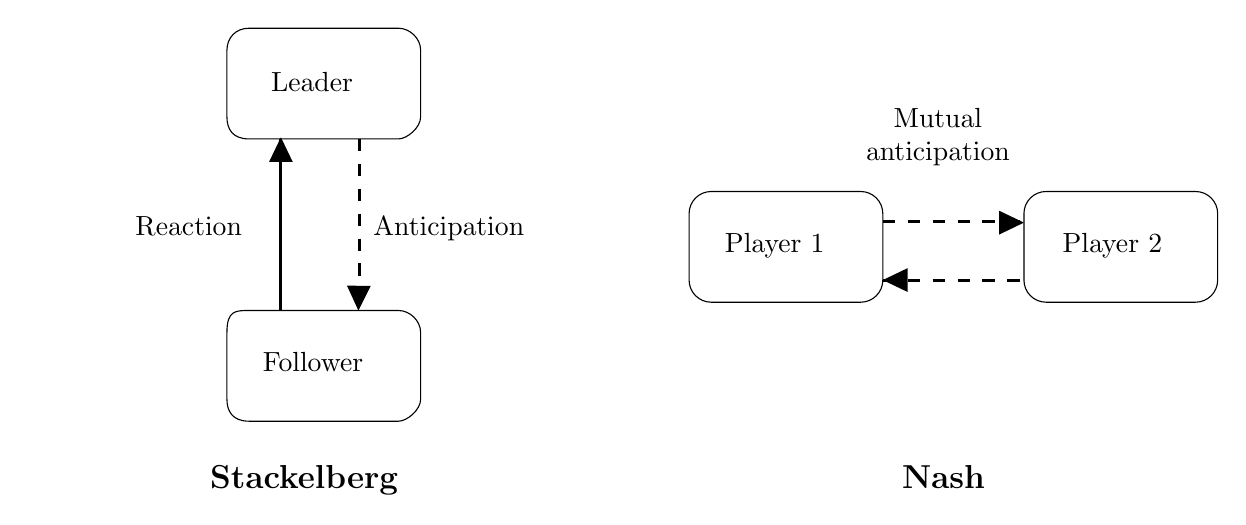
\begin{tikzpicture}[x=1pt,y=1pt,yscale=-1,xscale=1]
%uncomment if require:
\path (0,180); %set diagram left start at 0, and has height of 235
\draw   (72,48) .. controls (72,43.58) and (75,40) .. (80,40) -- (134,40) .. controls (138,40) and (142,43.58) .. (142,48) -- (142,72) .. controls (142,76) and (137,80) .. (134,80) -- (80,80) .. controls (74,80) and (72,76.42) .. (72,72) -- cycle ;
%Rounded Rect [id:dp668594301184202]
\draw   (72,150) .. controls (72,142) and (75,142) .. (80,142) -- (134,142) .. controls (138,142) and (142,145.58) .. (142,150) -- (142,174) .. controls (142,178) and (137,182) .. (134,182) -- (80,182) .. controls (74,182) and (72,178.42) .. (72,174) -- cycle ;
%Straight Lines [id:da7900936822479548]
\draw   [line width=1.1pt] (91.5,142) -- (91.5,80) ;
\draw [shift={(91.5,79.4)}, rotate = 450] [fill={rgb, 255:red, 0; green, 0; blue, 0 }  ][line width=0.08]  [draw opacity=0] (8.93,-4.29) -- (0,0) -- (8.93,4.29) -- cycle    ;
%Straight Lines [id:da3495843197611038]
\draw  [line width=1.1pt, dash pattern={on 4.5pt off 4.5pt}]  (120,80) -- (120,142) ;
\draw [shift={(119.5,142)}, rotate = 270.99] [fill={rgb, 255:red, 0; green, 0; blue, 0 }  ][line width=0.08]  [draw opacity=0] (8.93,-4.29) -- (0,0) -- (8.93,4.29) -- cycle    ;
%Rounded Rect [id:dp9652101194447742]
\draw   (239,107) .. controls (239,102.58) and (242.58,99) .. (247,99) -- (301,99) .. controls (305.42,99) and (309,102.58) .. (309,107) -- (309,131) .. controls (309,135.42) and (305.42,139) .. (301,139) -- (247,139) .. controls (242.58,139) and (239,135.42) .. (239,131) -- cycle ;
%Rounded Rect [id:dp09703506888751601]
\draw   (360,107) .. controls (360,102.58) and (363.58,99) .. (368,99) -- (422,99) .. controls (426.42,99) and (430,102.58) .. (430,107) -- (430,131) .. controls (430,135.42) and (426.42,139) .. (422,139) -- (368,139) .. controls (363.58,139) and (360,135.42) .. (360,131) -- cycle ;
%Straight Lines [id:da8121219380194096]
\draw [line width=1.1pt, dash pattern={on 4.5pt off 4.5pt}] (309,110) -- (359,110) ;
\draw [shift={(360,110.25)}, rotate = 180] [fill={rgb, 255:red, 0; green, 0; blue, 0 }  ][line width=0.08]  [draw opacity=0] (8.93,-4.29) -- (0,0) -- (8.93,4.29) -- cycle    ;
%Straight Lines [id:da0776548592195061]
\draw [line width=1.1pt, dash pattern={on 4.5pt off 4.5pt}] (309,131) -- (359,131) ;
\draw [shift={(309,131)}, rotate = 360] [fill={rgb, 255:red, 0; green, 0; blue, 0 }  ][line width=0.08]  [draw opacity=0] (8.93,-4.29) -- (0,0) -- (8.93,4.29) -- cycle    ;
% Text Node
\draw (84,156) node [anchor=north west][inner sep=0.75pt]   [align=left] {Follower};
% Text Node
\draw (87,55) node [anchor=north west][inner sep=0.75pt]   [align=left] {Leader};
% Text Node
\draw (251,113) node [anchor=north west][inner sep=0.75pt]   [align=left] {Player 1};
% Text Node
\draw (373,113) node [anchor=north west][inner sep=0.75pt]   [align=left] {Player 2};
\draw (302,68) node [anchor=north west][inner sep=0.75pt]   [align=center] {Mutual\\ anticipation};
\draw (65,197) node [anchor=north west][inner sep=0.75pt]   [align=left] {\large{\textbf{Stackelberg}}};
\draw (315,197) node [anchor=north west][inner sep=0.75pt]   [align=left] {\large{\textbf{Nash}}};
\draw (38,107) node [anchor=north west][inner sep=0.75pt]   [align=center] {Reaction};
\draw (124,107) node [anchor=north west][inner sep=0.75pt]   [align=center] {Anticipation};
\end{tikzpicture}
\caption{Structure of Stackelberg and Nash games}
\label{fig:stacknnash}
\end{figure}


On the contrary, \cref{fig:hello} is generated in advance by experiments and included
in the \textit{images} folder. Prefer including vectorial images, such as PDFs,
more than PNGs or JPEG that could appear with a low resolution.

\begin{figure}
  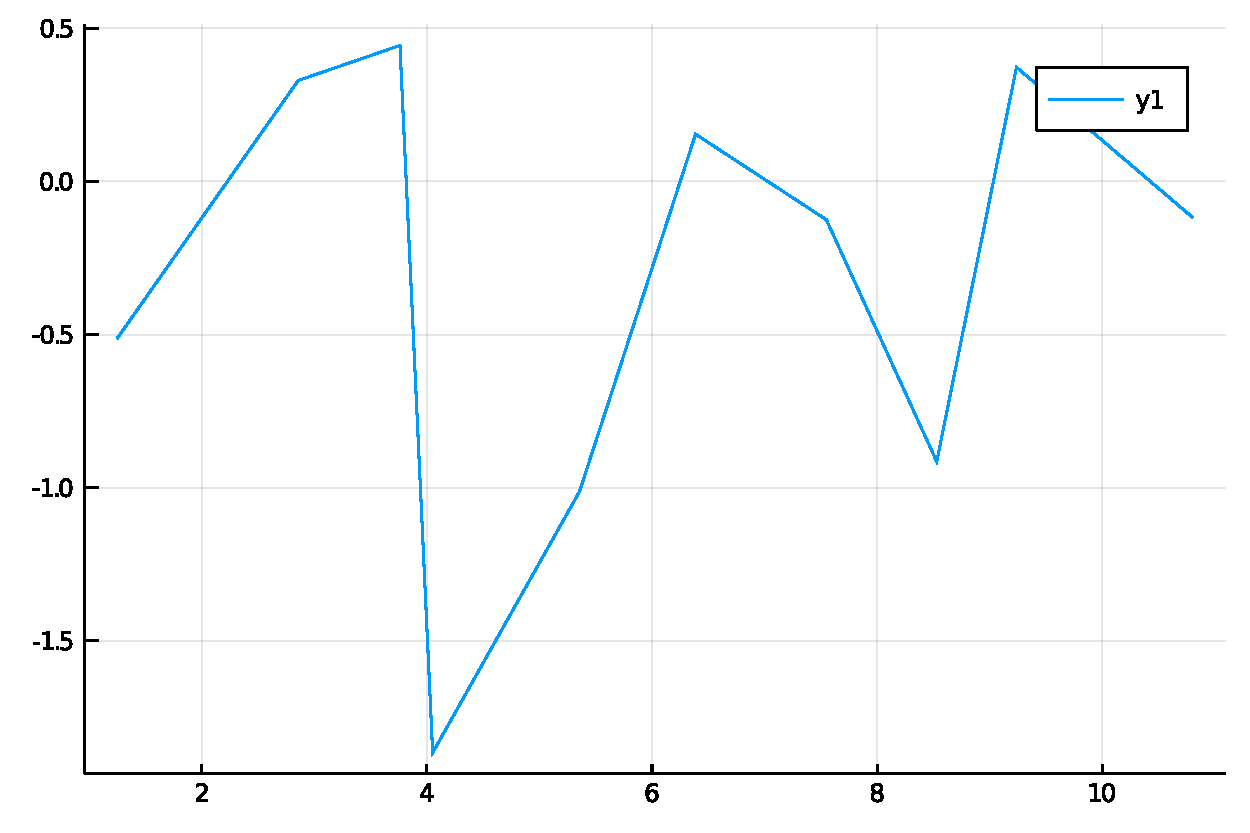
\includegraphics{hello}
  \caption{My ugly figure}
  \label{fig:hello}
\end{figure}

\section{Key concepts of the thesis}

This section provides the reader with broad explanations on the background and concepts from the thesis.
This is not yet a review of the relevant literature but a slower-paced explanation.
Ideally, this should be readable by people outside the direct thesis topic and equips them to understand the rest of the thesis.

\section{Research objectives}

We state in this section the research objectives, this does not need to be a detailed outline of the contribution chapters, since there is a dedicated chapter for this. (Summary of contributions)
